% Figure (S7): what the schedule choice is worth, relative to the review signal.
% y = gain from deliberate scheduling (S8 - S5) as a share of the review signal's
% value (S8 - S7), by horizon T and compounding rate eps; negative gains floored at
% zero (all within noise of zero). Default parameters otherwise; 64-200 seeds per
% cell (T_run_smooth horizon_growth + horizon_long, hash 21b0d9a; re-derived
% in-session, verify_s7.R). Curves for eps in {0.05, 0.15, 0.3, 0.55, 0.85};
% eps = 0.05, 0.15, 0.55 were swept to T = 5 only.
\begin{figure}[t]
\centering
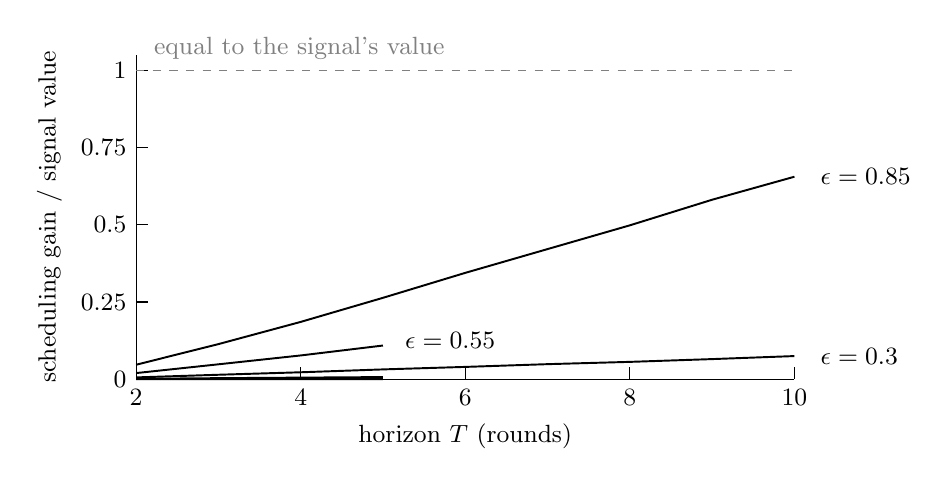
\begin{tikzpicture}
\begin{axis}[
  width=0.82\textwidth, height=5.7cm,
  axis lines*=left,
  xmin=2, xmax=10, ymin=0, ymax=1.05,
  xtick={2, 4, 6, 8, 10},
  ytick={0, 0.25, 0.5, 0.75, 1},
  yticklabels={0, 0.25, 0.5, 0.75, 1},
  xlabel={horizon $T$ (rounds)},
  ylabel={scheduling gain / signal value},
  ylabel style={font=\small}, xlabel style={font=\small},
  tick label style={font=\small},
  axis line style={line width=0.4pt},
  tick style={line width=0.4pt, black},
  clip=false,
]
\addplot[gray, dashed, line width=0.4pt, domain=2:10] {1};
\node[font=\small, gray, anchor=south west] at (axis cs:2.1,1.005) {equal to the signal's value};
\addplot[black, line width=0.7pt] coordinates {(2,0.0468) (3,0.1136) (4,0.1855) (5,0.2635) (6,0.3443) (7,0.4213) (8,0.4982) (9,0.5811) (10,0.6556)};
\addplot[black, line width=0.7pt] coordinates {(2,0.0198) (3,0.0482) (4,0.0769) (5,0.1090)};
\addplot[black, line width=0.7pt] coordinates {(2,0.0058) (3,0.0144) (4,0.0224) (5,0.0317) (6,0.0398) (7,0.0487) (8,0.0561) (9,0.0651) (10,0.0749)};
\addplot[black, line width=0.7pt] coordinates {(2,0.0012) (3,0.0034) (4,0.0051) (5,0.0069)};
\addplot[black, line width=0.7pt] coordinates {(2,0.0000) (3,0.0002) (4,0.0001) (5,0.0000)};
\node[font=\small, anchor=west] at (axis cs:10.2,0.656) {$\epsilon = 0.85$};
\node[font=\small, anchor=west] at (axis cs:5.15,0.126) {$\epsilon = 0.55$};
\node[font=\small, anchor=west] at (axis cs:10.2,0.075) {$\epsilon = 0.3$};
\end{axis}
\end{tikzpicture}
\caption{Choosing whom outweighs choosing when. The gain from deliberate scheduling
(a funder that plans its budget's spread over the horizon, over one that spends even
installments and re-decides each round) as a share of the review signal's value, by
horizon and compounding rate $\epsilon$; the default rate is $0.3$. In every setting
we test the gain is below the signal's value: an order of magnitude below or more at
the default rate and below, and approaching the signal's value only at the joint
extreme of the highest rate and the longest horizon. The two lowest curves, at $\epsilon = 0.15$ and $0.05$, and the curve at $0.55$ were
swept to five rounds.}
\label{fig:schedule-vs-signal}
\end{figure}
